\documentclass[tikz]{standalone}
\usetikzlibrary {automata,positioning,fit,calc} 
\usepackage{inconsolata}
\begin{document}
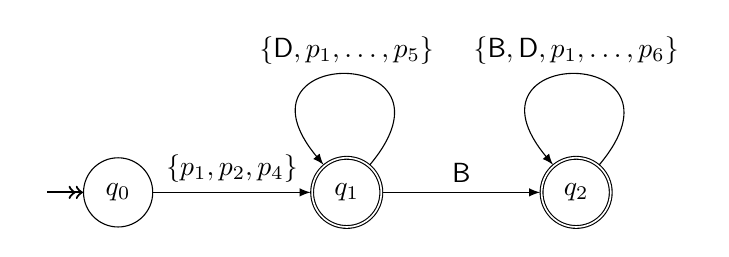
\begin{tikzpicture}[every initial by arrow/.style={text={},->>,thick},-latex,initial text={},node distance=2cm]


%%%%%%%%%%%%%%%%%%%%%% PRECEDENCE

\node[state,initial] (q03A) {$q_0$};
\node[state,accepting,right=of q03A] (q03V) {$q_1$};
\draw[-latex] (q03A) edge node[above] {$\{p_1,p_2,p_4\}$} (q03V);
%\path[-latex,draw] (q03V) to  [in=130,out=50,loop,-latex,distance=1cm] node[above] {$\textsf{C}$} (q03V);
\path[-latex,draw] (q03V) to  [in=130,out=50,loop,-latex,distance=2cm] node[above] (e1) {$\{\textsf{D},p_1,\dots,p_5\}$} (q03V);


        
\node[state,accepting,right=of q03V] (q13V) {$q_2$};
\draw[-latex] (q03V) edge node[above] {$\textsf{B}$} (q13V);
%\path[-latex,draw] (q13V) to  [in=130,out=50,loop,-latex,distance=1cm] node[above] {$\textsf{A}$} (q13V);
\path[-latex,draw] (q13V) to  [in=130,out=50,loop,-latex,distance=2cm] node[above](e2) {$\{\textsf{B},\textsf{D},p_1,\dots,p_6\}$} (q13V);

%\path[-latex,draw] (q13V) to  [in=230,out=320,loop,-latex,distance=1cm] node[above] {$\textsf{C}$} (q13V);
%\path[-latex,draw] (q13V) to  [in=230,out=320,loop,-latex,distance=2cm] node[above] (e4) {$\textsf{D}$} (q13V);

\coordinate (PR) at ($(q13V)+(1,2)$) ;
\coordinate (PR3) at ($(q13V)+(1,-2)$) ;


\end{tikzpicture}
\end{document}